\section{Quark Level Corrections additional details}
\label{sec:AppQLCs}

As mentioned in the main text, due to the different quark-level cuts used in this iteration of the analysis compared to the PR2 one, the QLCs are re-evaluated for the \BpmKpmJpsi and \BsJpsiPhi samples.  
To do this, dedicated unbiased and quark-biased samples are generated for each of these samples without any final state cuts. 
For \BpmKpmJpsi, the QLCs are evaluated using only \BpKpJpsi as charge conjugation is assumed not to effect the kinematics at truth level. 
For each of the biased and unbiased, approximately 10~million events are generated in order to ensure good statistics and small uncertainties. 
The values and relative uncertainties of the re-evaluated QLCs are shown in Figures~\ref{fig:BpJpsiKpQLCs} and~\ref{fig:BsJpsiPhiQLCs} for \BpKpJpsi and \BsJpsiPhi respectively. 

\begin{figure}[h]
    \centering
    \subfloat[\BpKpJpsi QLCs values]{
        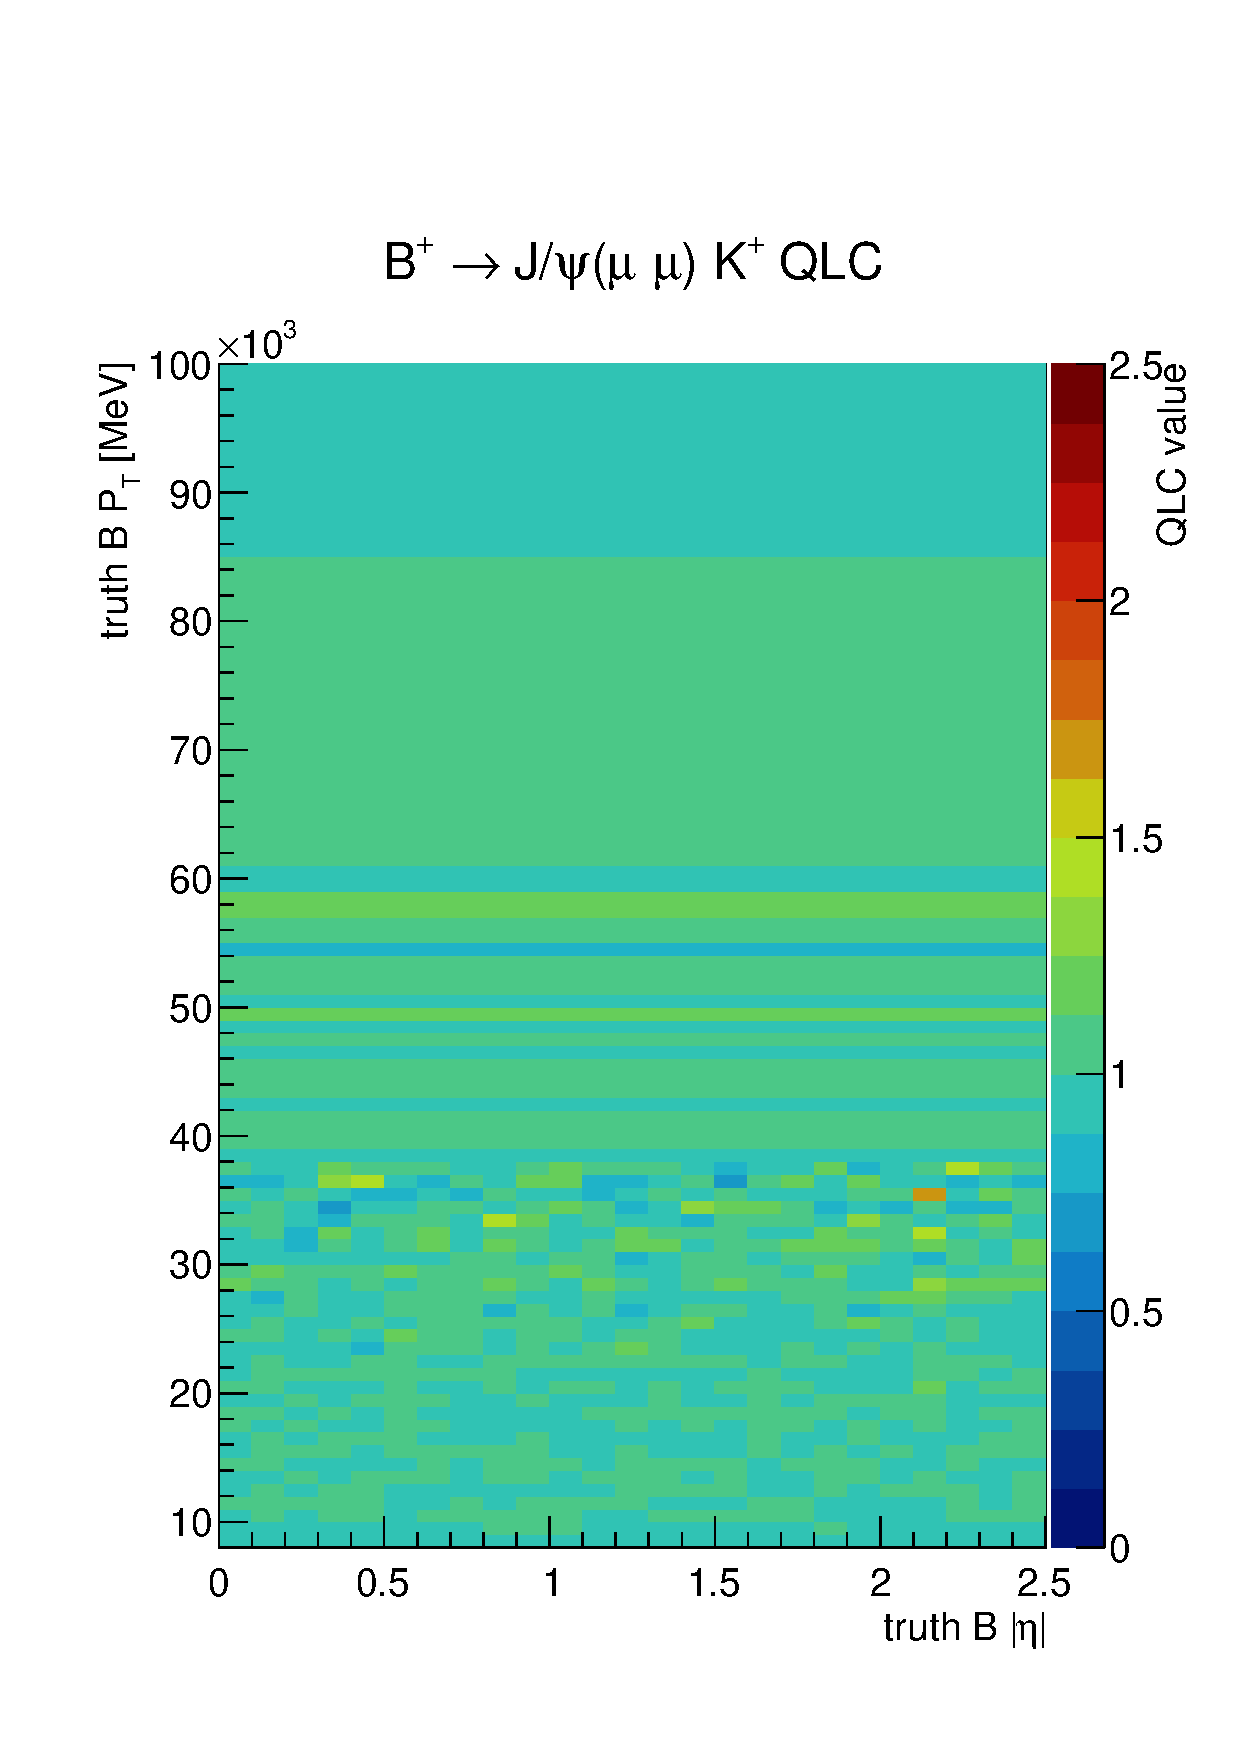
\includegraphics[width=0.45\textwidth]{figures/QLCs/BpToJpsiKplus_10M/ActualQLC.pdf}
        \label{fig:BpKpJpsiQLC_vals}
    }
    \subfloat[\BpKpJpsi QLCs relative uncertainties]{
        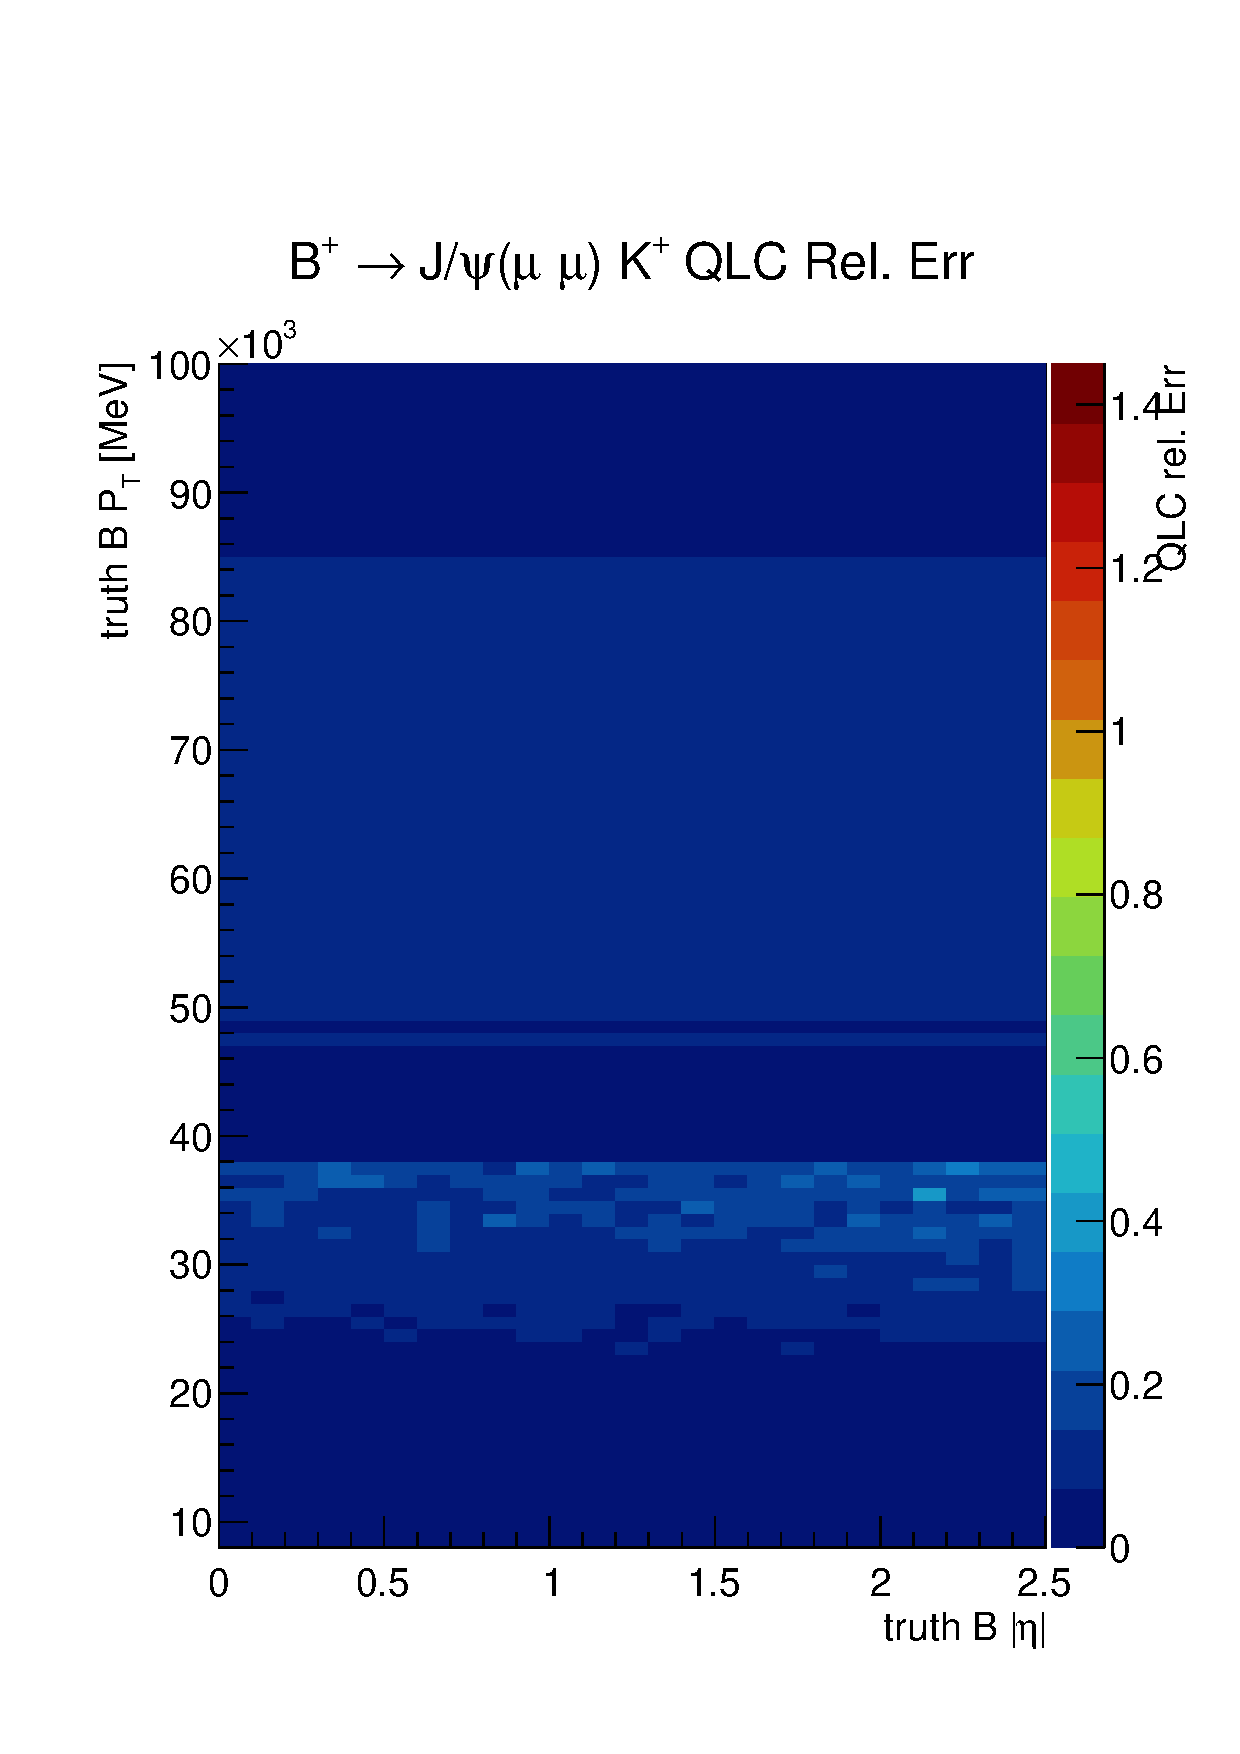
\includegraphics[width=0.45\textwidth]{figures/QLCs/BpToJpsiKplus_10M/QLCErr.pdf}
        \label{fig:BpKpJpsiQLC_errs}
    }
    \caption{Re-evaluated QLCs and uncertainties for \BpKpJpsi}
    \label{fig:BpJpsiKpQLCs}
\end{figure}

\begin{figure}[h]
    \centering
    \subfloat[\BsJpsiPhi QLCs values]{
        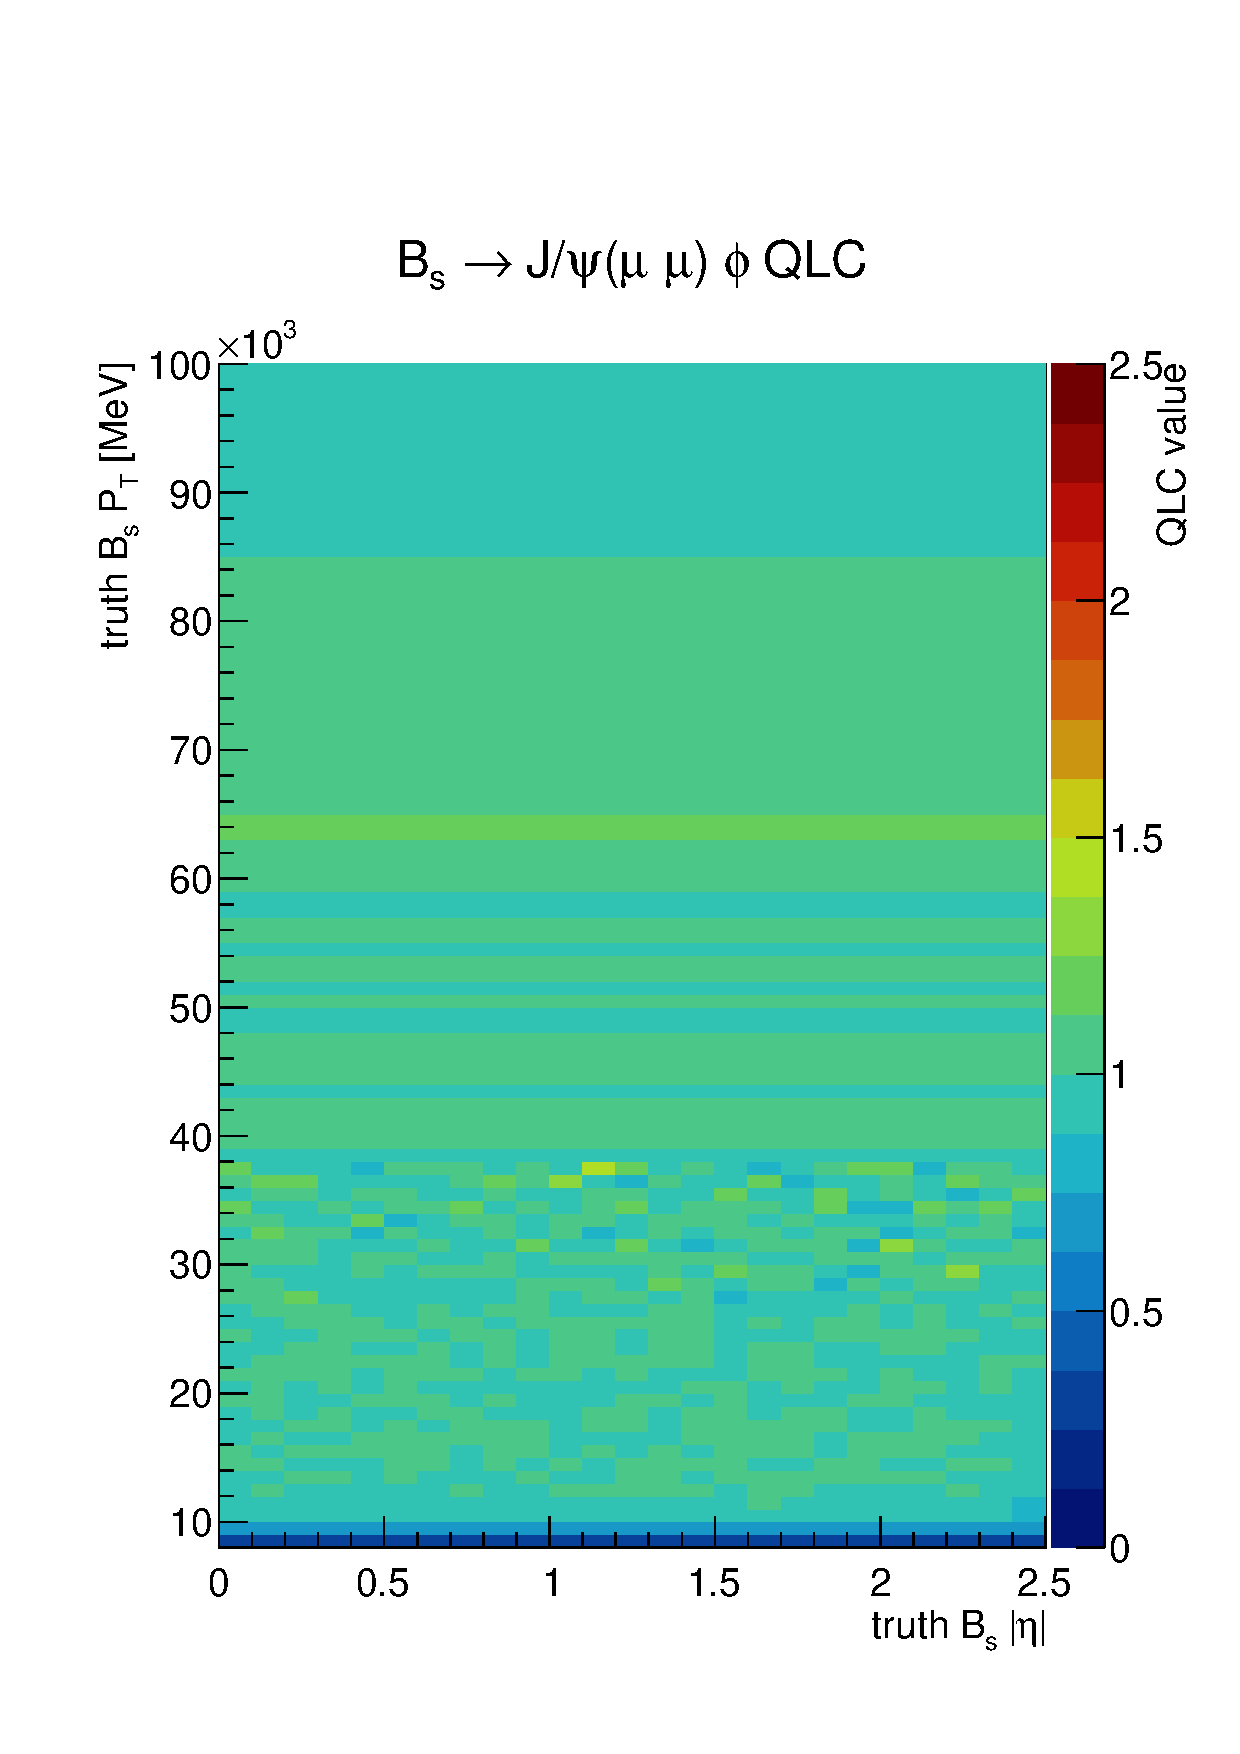
\includegraphics[width=0.45\textwidth]{figures/QLCs/BsToJpsiPhi_10M/ActualQLC.pdf}
        \label{fig:BsJpsiPhiQLC_vals}
    }
    \subfloat[\BsJpsiPhi QLCs relative uncertainties]{
        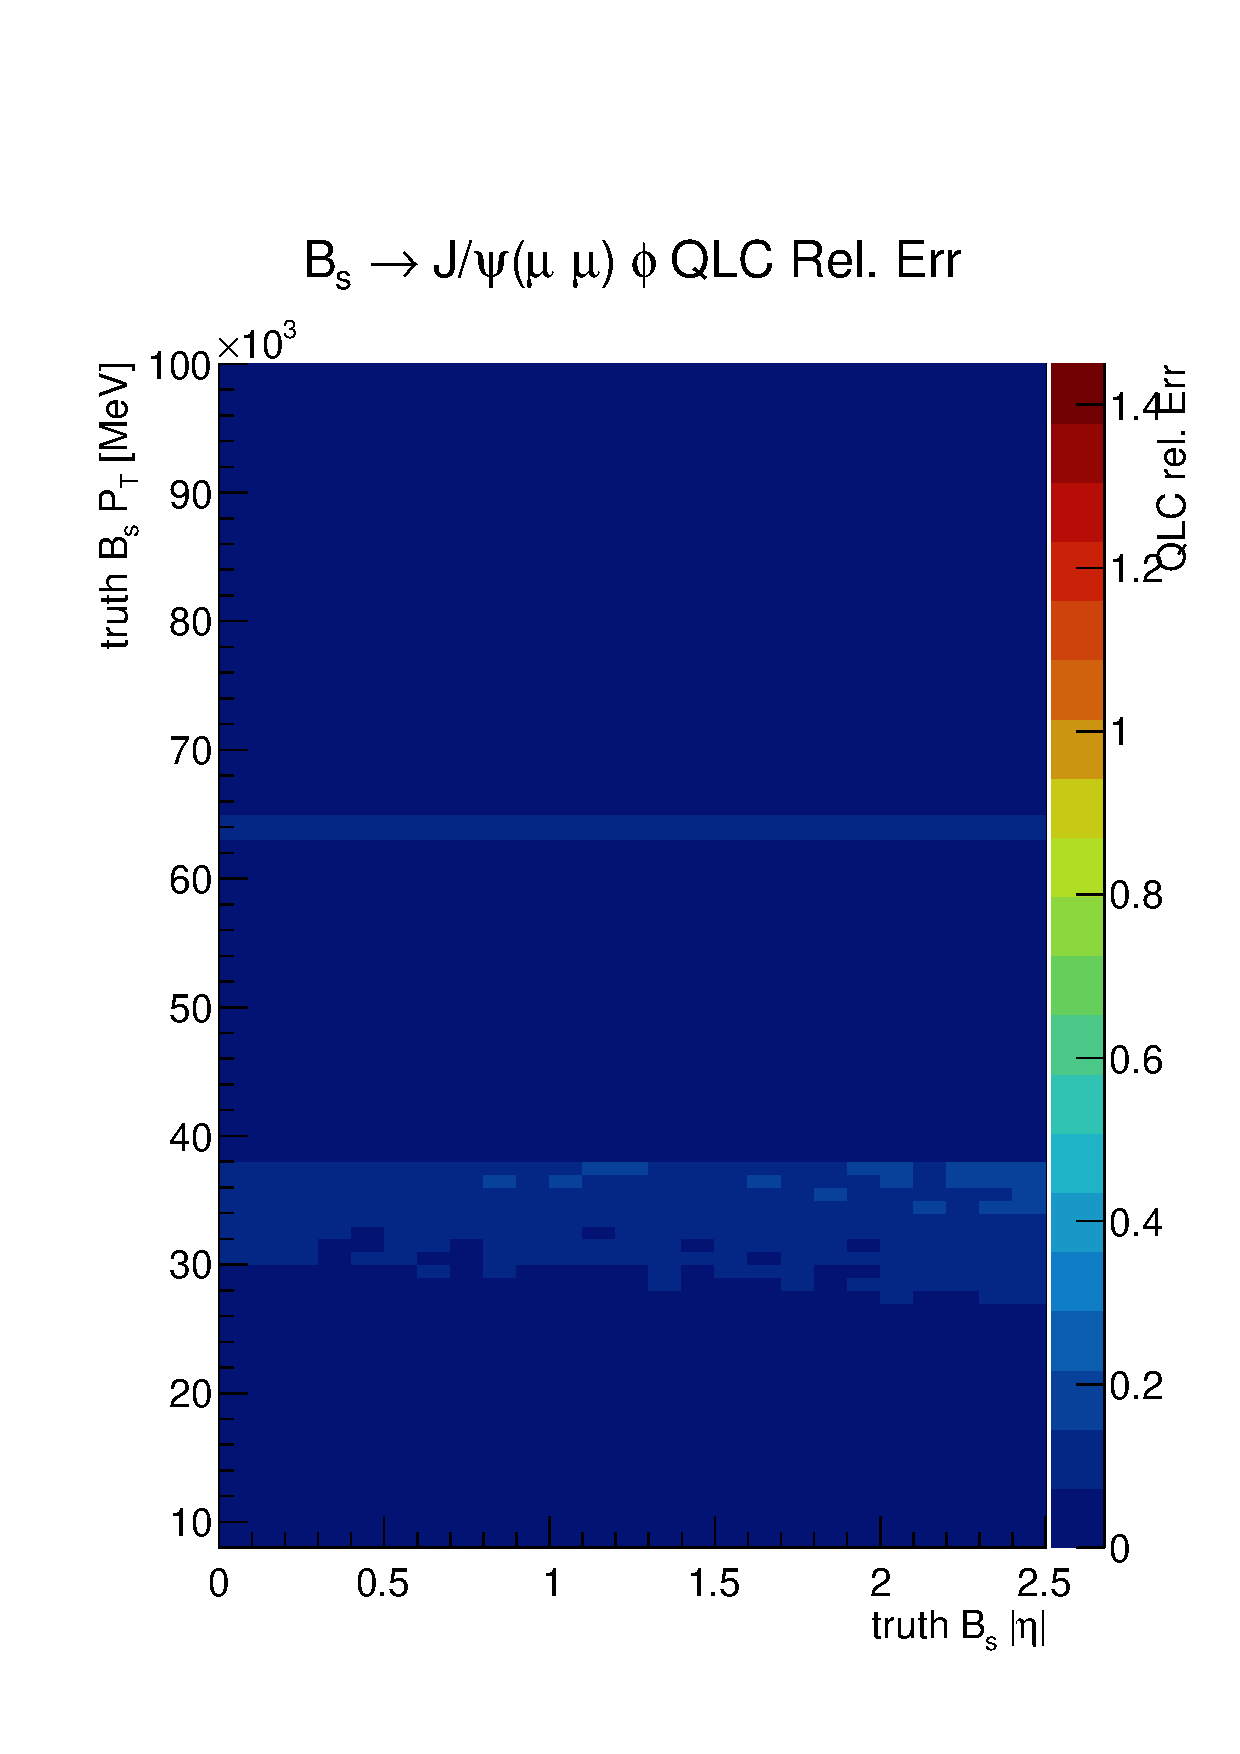
\includegraphics[width=0.45\textwidth]{figures/QLCs/BsToJpsiPhi_10M/QLCErr.pdf}
        \label{fig:BsJpsiPhiQLC_errs}
    }
    \caption{Re-evaluated QLCs and uncertainties for \BpKpJpsi}
    \label{fig:BsJpsiPhiQLCs}
\end{figure}
\clearpage
